\section{Electrons}
\label{sec:id-electron}

The electron candidates used in this analysis are
taken from GSF electron candidates, which are 
reconstructed according to the
process described in Section \ref{sec:reco-electron}.
On top of the selection applied during reconstruction,
a further electron identification selection is applied to 
reduce contamination from
various backgrounds.
This additional identification is referred to as the v3.1
high energy electron pair (HEEP) ID, 
\nomenclature{HEEP}{High energy electron pair identification}
and it was originally developed for an analysis searching for a $Z'$ resonance
decaying to two electrons \cite{zprime-2011}.
Significant backgrounds include electrons produced within jets,
electrons from photon conversion,
and various physics objects (jets, for example) that are 
misreconstructed as electrons.  These misreconstructed objects
are referred to as ``fake electrons''.
Since the $Z'$ search used the HEEP ID to identify high energy electrons, many searches for heavy,
exotic physics processes with a final state of high energy electrons (including 
first generation leptoquarks) use the HEEP ID also.

Differences in selection aside, the main difference
between HEEP electrons and GSF electrons comes from the energy measurement.
The energy measurement for GSF electrons is a weighted average
of the energy value obtained from the GSF fit and the energy value obtained from the supercluster.
The energy measurement for HEEP electrons comes purely from the supercluster.
The weighted average gives better performance for low energy electrons ($\et < 15$ GeV)
but for electrons with $\et > 25$ GeV, the weighted average is dominated
by the supercluster measurement and the two methods yield effectively identical results.
In certain rare situations, however, it is possible for the weighted average to discard
the supercluster measurement completely and use the GSF track measurement alone.  This can
result in low-energy electrons mistakenly being assigned very high energy measurements.
HEEP electrons use only the supercluster energy by default in order to avoid this situation.
In addition to passing the HEEP ID,
electrons in this analysis are required to have $\et > 40$ GeV.

The HEEP ID is a cut-based ID, and the contributing variables are 
described below.
The numerical requirements for each of these variables are shown
in Table \ref{tab:heep}.

\begin{table}
  \centering
  \small
  \begin{tabular}{ c|c|c } 
    Variable & Barrel (EB) criterion & Endcap (EE) criterion \\
    \hline\hline
    $\et$                        & $>$ 30~\GeV & $>$ 30~\GeV \\
    $|\eta_{\text{SC}}|$                    & $|\eta|< 1.442$      & $|\eta|> 1.56$ \\
    ecalDrivenSeed() & $=1$ & $=1$ \\
    \dEtaIn                    & $< 0.005$ & $< 0.007$ \\
    \dPhiIn                    &  $< 0.09$  & $< 0.09$ \\
    \HoE                        & $<0.05$    & $<0.05$ \\
    \SigmaiEtaiEta      &  -            & $<0.03$ \\
    \ETwoEFive          &  $>0.94$ OR  \EOneEFive $> 0.83$ & - \\
    \EMIso + \HADIsoOne & $< 2+0.03 \times \et$ GeV &  $<2.5$ GeV (for $\et<50$ GeV) \\
    &                                            &  $<2.5+0.03 \times (\et-50)$ GeV (for $\et>50$ GeV) \\
    \HADIsoTwo         &   -  &  $<0.5$ \\
    \TRKIso                 & $<7.5$~\GeV & $<15$~\GeV \\
    Inner Layer Lost Hits  & $=0$ & $=0$ \\ 
  \end{tabular}
  \caption{The ``HEEP v3.1'' selection criteria for electron ID and isolation.}
  \label{tab:heep}
\end{table}



\begin{itemize}
  \item {\bf \et:} the transverse energy of the electron. \et~is defined
    as the calibrated energy measurement from the ECAL supercluster
    multiplied by $\text{sin}(\theta_{\text{track}})$, where $\theta_{\text{track}}$
    is the polar angel of the electron GSF track measured at the inner layer of the 
    inner tracker and extrapolated to the $pp$ interaction vertex.    
  \item {\bf $\eta_{\text{SC}}$:} the pseudorapidity of the supercluster 
    used to reconstruct the electron candidate.  
    Electrons with $|\eta_{\text{SC}}| < 1.442$ are identified as electrons from the EB.
    Electrons with $1.560 < |\eta_{\text{SC}}| < 2.5$ are identified as electrons from the EE.
    Electrons with any other value of $|\eta_{\text{SC}}|$ are not considered for this analysis.
    This requirement excludes electrons that are reconstructed near the gap between the EB and the EE,
    where the reconstruction efficiency and energy resolution are poor.
    This gap is illustrated in Figure \ref{fig:ecal}.
  \item {\bf Electron seeding algorithm.}  Two electron seeding algorithms are used in CMS:
    ECAL-driven and tracker-driven.  Both seeding algorithms are described in Section \ref{sec:reco-electron}.
    Only electrons that are purely ECAL-driven or both ECAL-driven and tracker-driven are considered for this analysis.
    There are two reasons for this requirement.  First, ECAL-driven
    electrons are compatible with the L1 trigger, which uses ECAL-driven measurements to select
    events with high energy electrons.  Second, at the time of this analysis, 
    only ECAL-driven reconstruction had been validated for the high energy electrons used in this analysis.
  \item {\bf \dEtaIn:} the difference between the value of $\eta$ taken from the GSF track
    measured at the inner layer of the inner tracker and extrapolated to the $pp$ interaction vertex
    and the value of $\eta$ taken from the electron's supercluster ($\eta_{\text{SC}}$).
    \dEtaIn~is required to be close to zero.
  \item {\bf \dPhiIn:} the difference between the value of $\phi$ taken from the GSF track
    measured at the inner layer of the inner tracker and extrapolated to the $pp$ interaction vertex
    and the value of $\phi$ taken from the electron's supercluster ($\phi_{\text{SC}}$).
    \dPhiIn~is required to be close to zero.
  \item {\bf \HoE:} ratio between the energy measured by the HCAL within a cone of radius 
    $\sqrt{\Delta\phi^2\times\Delta\eta^2} = 0.15$ centered on the electron's supercluster position
    and the energy of the electron's supercluster.  \HoE~is required to be small.
  \item {\bf \SigmaiEtaiEta:} a measure of the spread in pseudorapidity of the electron energy
    within a $5\times5$ block of ECAL crystals, centered on the seed crystal.  As mentioned
    in Section \ref{sec:reco-electron}, the spread of the electron energy 
    is expected to be narrow in pseudorapidity, so \SigmaiEtaiEta~is required to be small.
  \item {\bf \ETwoEFive:} the fraction of the total electron energy contained within a block 
    of 2 crystals (in $\eta$) $\times$ 5 crystals (in $\phi$).  \ETwoEFive~is required to be large 
    in order to remove electrons that are contained within jets.
  \item {\bf \EOneEFive:} the fraction of the total electron energy contained within a block 
    of 1 crystal (in $\eta$) $\times$ 5 crystals (in $\phi$).  \EOneEFive~is required to be large 
    in order to remove electrons that are contained within jets.
  \item {\bf ECAL isolation: } the sum of the transverse energy of all EB RecHits with 
    $E > 0.08$ GeV and all EE RecHits with $E > 0.1$ GeV within a cone of radius 
    $\sqrt{\Delta\phi^2\times\Delta\eta^2} = 0.3$ centered around the electron's position in the ECAL.
    An inner cone with a radius of three crystals and an $\eta$ strip of width 3 crystals is excluded from
    this sum.  ECAL isolation is required to be small in order to remove electrons that are contained
    within jets.
  \item {\bf HCAL depth 1 isolation:} the sum of the HCAL ``depth 1'' RecHits within a cone 
    of $\sqrt{\Delta\phi^2\times\Delta\eta^2} = 0.3$ centered on the electron's position in the ECAL.
    HCAL RecHits within a cone of $\sqrt{\Delta\phi^2\times\Delta\eta^2} = 0.15$ are excluded from this
    sum.  In this context, depth 1 is defined as all depths for HCAL towers 1-17, depth 1 for towers 
    18-29, and depth 2 for towers 27-29.  The depth segmentation of the HCAL is described in Section
    \ref{sec:hcal} and shown in Figure \ref{fig:hcal-segmentation}.  HCAL depth 1 isolation is 
    required to be small in order to remove electrons that are contained
    within jets.
  \item {\bf HCAL depth 2 isolation:} the sum of the HCAL ``depth 2'' RecHits within a cone 
    of $\sqrt{\Delta\phi^2\times\Delta\eta^2} = 0.3$ centered on the electron's position in the ECAL.
    HCAL RecHits within a cone of $\sqrt{\Delta\phi^2\times\Delta\eta^2} = 0.15$ are excluded from this
    sum.  In this context, depth 2 is defined as all depths that are not included in depth 1
    for towers 18-29. The depth segmentation of the HCAL is described in Section
    \ref{sec:hcal} and shown in Figure \ref{fig:hcal-segmentation}. HCAL depth 2 isolation is 
    required to be small in order to remove electrons that are contained
    within jets.
  \item {\bf Tracker isolation:} the sum of the \pt~of the tracks within a cone
    of radius $\sqrt{\Delta\phi^2\times\Delta\eta^2} = 0.3$ centered around the GSF track at the interaction
    point having $\pt > 0.7$~GeV and 
    $z_0$ within 0.2 cm of the $z_0$ of the electron's GSF track.
    Tracks within a cone of $\sqrt{\Delta\phi^2\times\Delta\eta^2} = 0.04$ of the GSF track at the interaction
    point are not considered.  The variable $z_0$ is defined as the minimum distance in $z$ from the
    point (0,0,0).  Tracker isolation is 
    required to be small in order to remove electrons that are contained
    within jets.
\begin{figure}
  \centering
  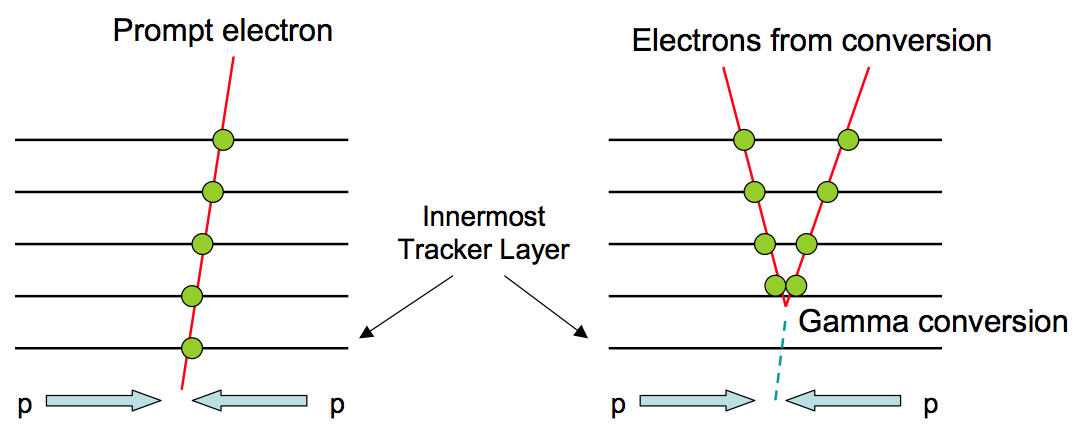
\includegraphics[width=0.6\textwidth]{tex/analysis/object_selection/fig/heep-conversions.png}
  \caption{
    Prompt electrons originating from the primary $pp$ collision vertex (left) usually have
    ``hits'' on the innermost layer of the inner tracker.  Conversely, electrons from
    converted photons (right) often do not have hits on the innermost layer of the inner tracker.
  }
  \label{fig:heep-conversions}
\end{figure}
  \item {\bf Missing tracker hits:} the number of expected hits in the inner tracker that are missing from a GSF track.
    As shown in Figure \ref{fig:heep-conversions}, electrons that are produced from photon conversions often have
    missing hits in the first layer of the inner tracker.  For this reason, the HEEP ID requires electrons
    to have zero missing tracker hits.
\end{itemize}

